\chapter{Исследовательская часть}

В данном разделе поставлена задача исследования зависимостей среднего времени выполнения запроса, числа запросов в секунду, средней скорости передачи данных и средней скорости передачи данных на одно соединение от количества активных соединений.
\section{Характеристики устройства}

Исследования проводились на машине со следующими характеристиками:
\begin{itemize}[label=---]
	\item процессор Intel(R) Core(TM) i5-10210U, тактовая частота 1.60 ГГц, 8 логических ядер;
	\item оперативная память: 16~ГБ;
	\item операционная система: Ubuntu 22.04.4 LTS.
\end{itemize}

\section{Методика исследования}

Для проведения исследования использовалась утилита wrk~\cite{ubuntu_wrk}, позволяющая получить необходимые метрики при заданном числе активных соединений. Параметры тестового прогона:
\begin{itemize}
	\item адрес сервера: \texttt{localhost:8080};
	\item размер запрашиваемого ресурса: 5~МБ;
	\item количество создающих нагрузку потоков: 4;
	\item число активных соединений: от 50 до 1050 или первой ошибки запроса с шагом 100;
	\item число процессов-обработчиков: 4, 8, 16;
	\item длительность нагрузки при заданном числе обработчиков и активных соединений: 8~с;
	\item количество замеров при заданном числе обработчиков и активных соединений: 10.
\end{itemize}

\section{Результаты}

Основным ограничением максимального числа открытых соединений является ограничение на номера файловых дескрипторов \texttt{FD\_SETSIZE} (1024). Таким образом при 1050 активных соединениях происходит 31 ошибка установки соединения, из-за недостаточного количества номеров свободных файловых дескрипторов.

Полученные зависимости представлены на графиках:
\begin{itemize}
	\item рисунок~\ref{fig:latency}~---~зависимость среднего времени числа выполнения запроса от числа активных соединений;
	\item рисунок~\ref{fig:rps}~---~зависимость RPS от числа активных соединений;
	\item рисунок~\ref{fig:speed}~---~зависимость средней скорости передачи данных от числа активных соединений;
	\item рисунок~\ref{fig:speedPerOne}~---~зависимость средней скорости передачи данных на одно соединение от числа активных соединений.
\end{itemize}



\begin{figure}[H]
	\centering
	
\includegraphics[width=0.9\textwidth]{images/latency_vs_clients.pdf}
	\caption{Зависимость среднего времени выполнения запроса от числа активных соединений}
	\label{fig:latency}
\end{figure}

\begin{figure}[H]
	\centering
	
\includegraphics[width=0.9\textwidth]{images/rps_vs_clients.pdf}
	\caption{Зависимость RPS от числа активных соединений}
	\label{fig:rps}
\end{figure}

\begin{figure}[H]
	\centering
	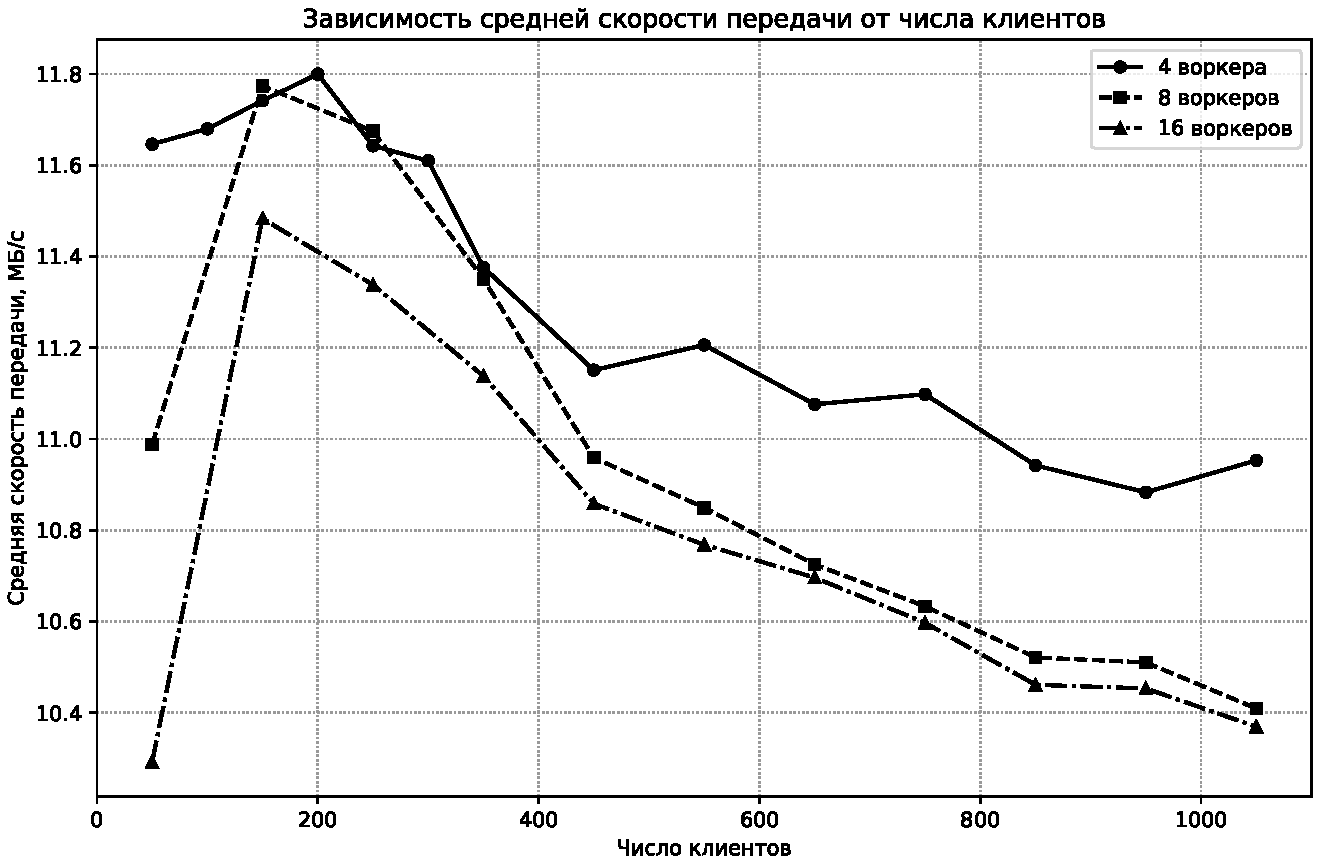
\includegraphics[width=0.9\textwidth]{images/transfer_vs_clients.pdf}
	\caption{Зависимость средней скорости передачи данных от числа активных соединений}
	\label{fig:speed}
\end{figure}

\begin{figure}[H]
	\centering
	
\includegraphics[width=0.9\textwidth]{images/per_connection_speed_vs_clients.pdf}
	\caption{Зависимость средней скорости передачи данных на одно соединение от числа активных соединений}
	\label{fig:speedPerOne}
\end{figure}

\section{Вывод}

По результатам замеров исследования можно сделать следующие выводы:
\begin{itemize}
	\item среднее время выполнения запроса увеличивается с ростом числа активных соединений, от менее 5 мс при 50 соединениях до приблизительно 23 мс при 1000 соединениях;
	\item минимальная скорость роста времени выполнения запроса наблюдается при 16 процессах-обработчиках;
	\item расхождение во времени выполнения процесса при 1000 активных соединениях между максимальным значением при 4 обработчиках и минимальным при 16 составляет не более 3 мс;
	\item количество обрабатываемых запросов в секунду уменьшается с ростом числа активных соединений от порядка 23000 RPS при 150 соединениях до порядка 20800 RPS при 1000 соединениях;
	\item минимальное значение RPS при 1000 активных соединений наблюдается при 16 процессах-обработчиках, максимальное~---~при 4;
	\item средняя скорость передачи данных также уменьшается с ростом числа активных соединений от порядка 11.5 МБ/с при 150 соединениях до 10.4 МБ/с при 1000 соединениях;
	\item максимальное значение скорости передачи данных при 1000 активных соединениях наблюдается при 4 процессах-обработчиках, минимальное при 16;
	\item средняя скорость передачи данных на одно соединение убывает с ростом числа активных соединений от порядка 210 КБ/с при 50 соединениях до порядка 10 КБ/с при 1000 соединениях;
	\item различия в скорости передачи данных на одно соединение при количестве активных соединений свыше 250 не превышает 2 КБ/с.
\end{itemize}


\clearpage